\newpage

\section*{ $^{55}$Mn(n,$\gamma$)$^{56}$Mn }

Power Level: 100 kW(th) \\
Time at Power: 60.0 s \\
Wait Time:  2.0 h \\
Counting Time: 10.0 m \\
Total Activity at Removal: 6.40e+01 $\mu Ci$

\begin{table*}[h]
\centering
\begin{tabular}{ |c|c|c|c|c|c| }
 \hline
 Position & Mass $mg$ & Counting Activity $\mu Ci$ & Area (Counts) & Error \% \\
 \hline 
 1 & 1.08 & 7.87e+00 & 3.65e+05 & 0.1656 \\ 
\hline
 2 & 1.08 & 1.15e+01 & 5.35e+05 & 0.1368 \\ 
\hline
 3 & 1.08 & 1.02e+01 & 4.74e+05 & 0.1453 \\ 
\hline
 4 & 1.08 & 5.69e+00 & 2.64e+05 & 0.1947 \\ 
\hline
\end{tabular}
\end{table*}

\begin{figure}[h]
\centering
\begin{subfigure}{.5\textwidth}
  \centering
     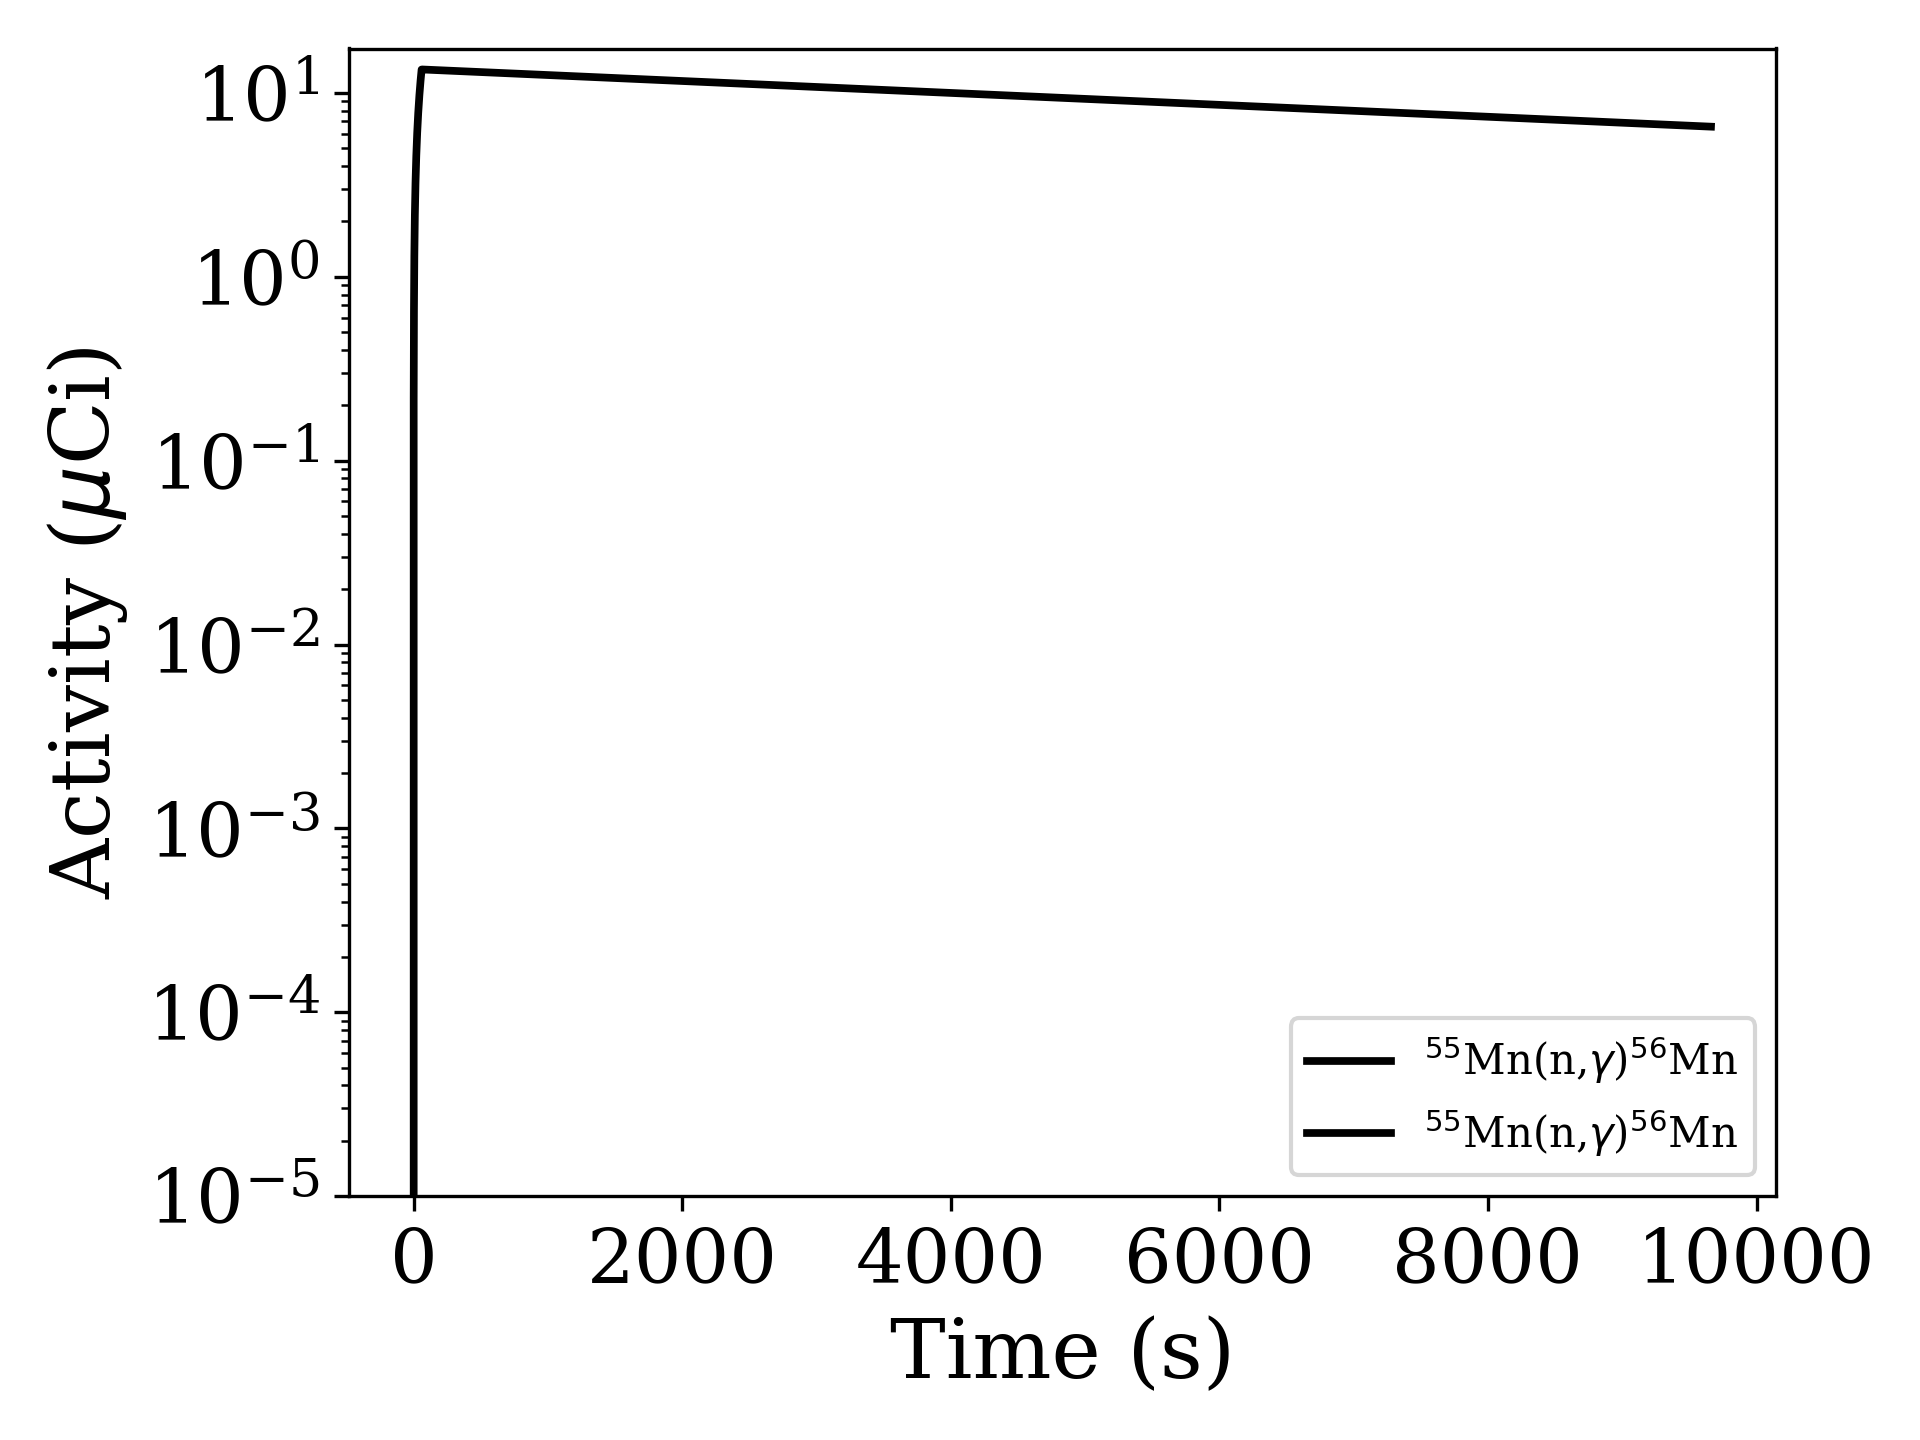
\includegraphics[width=.8\textwidth]{plot/Mn-55(n,gamma)Mn-56_library1} 

  \caption{A subfigure}
  \label{fig:sub1}
\end{subfigure}%
\begin{subfigure}{.5\textwidth}
  \centering
     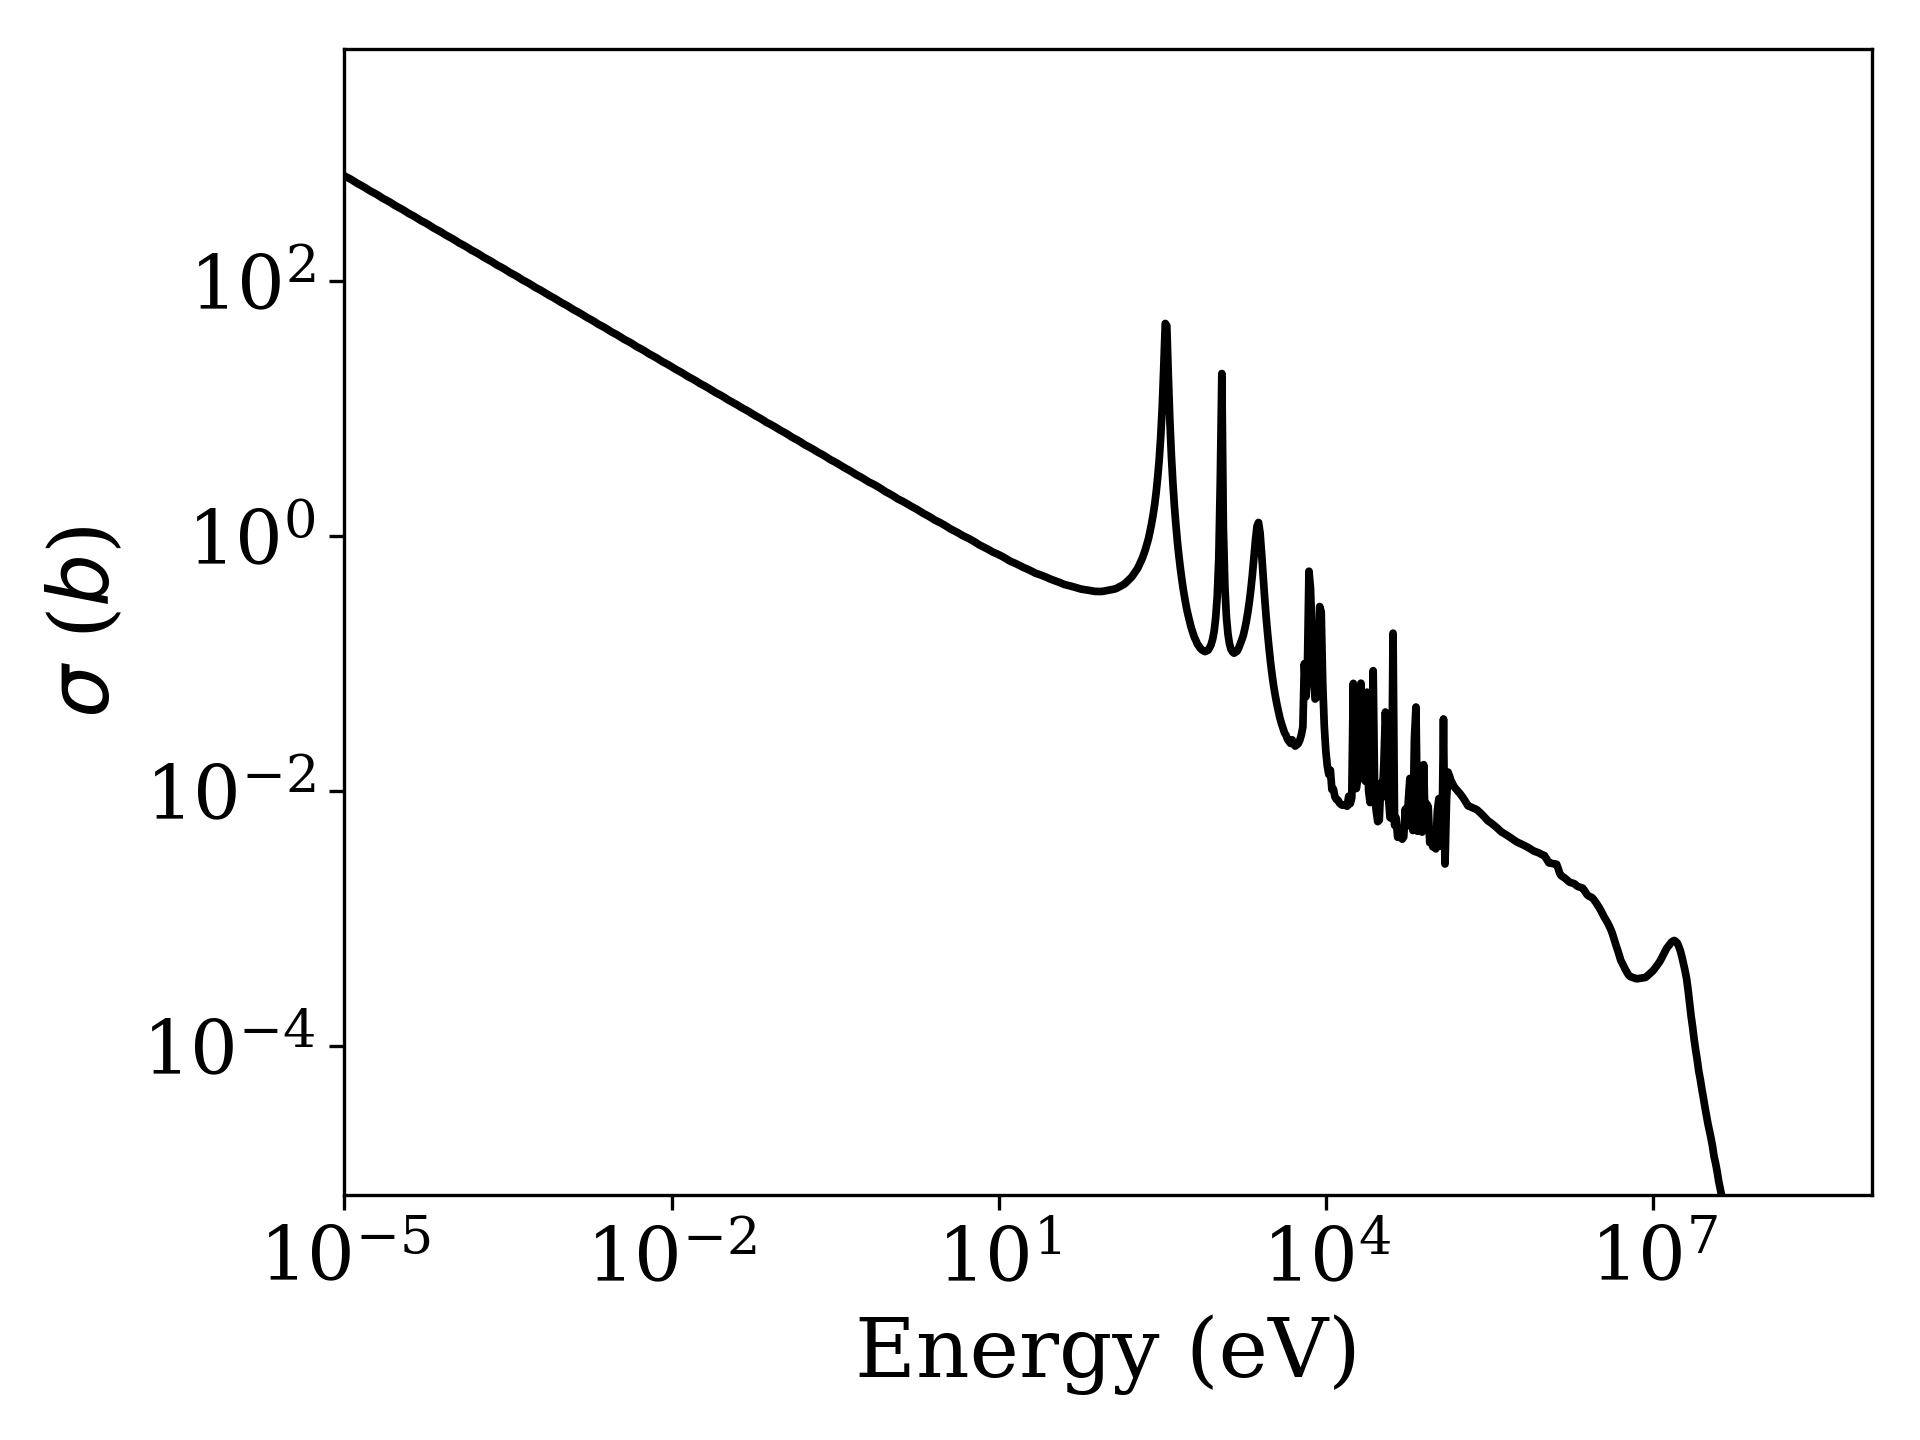
\includegraphics[width=.8\textwidth]{plot/Mn-55(n,gamma)Mn-56} 

  \caption{A subfigure}
  \label{fig:sub2}
\end{subfigure}
\caption{A figure with two subfigures}
\label{fig:test}
\end{figure}

\begin{table*}[h]
\centering
\begin{tabular}{ |c|c|c|c|c|c|c| }
 \hline
 Reaction & T$_{1/2}$ & ROI (eV) & Important Gammas (keV) \\
 \hline 
 $^{55}$Mn(n,$\gamma$)$^{56}$Mn &  2.6 h & 6.95e-03, 3.29e+02 & 1810.726(0.269) \\ 
\hline
\end{tabular}
\end{table*}
